\section{Umsetzung}

In diesem Kapitel wird die Demo-App \textbf{ARMarbleRun} beschrieben, die im Rahmen dieses Projekts erstellt wurde.
Der Code der App, genauso wie der Prototypen, ist auf GitHub unter \url{https://github.com/eduDorus/PAWI} frei verfügbar.

\subsection{Konzept}

Zur Illustration der Möglichkeiten der AR Technologie soll eine lauffähige iOS Demo-App entstehen.
Im Abschnitt zur Lösungswahl (\ref{sub:loesungswahl}) wurde anhand der erarbeiteten Prototypen entschieden, dass die App primär zwei Anwendungsfälle enthalten soll:

\begin{itemize}
	\item Eine interaktive Bauanleitung, bei der eine virtuelle Kugelbahn in Augmented Reality als Anleitung für den Benutzer zum Bau der physischen Kugelbahn verwendet wird.
	\item Der Bau und die Bearbeitung von virtuellen Kugelbahnen in Augmented Reality.
\end{itemize}

Eine ausführliche Architekturdokumentation findet sich im Anhang \ref{appendix:architekturdokumentation}.
Darin enthalten sind die kompletten Funktionalen Anforderungen als User Stories mit Akzeptanzkriterien (\ref{appendix:funktionale-anforderungen}) und Nichtfunktionalen Anforderungen (\ref{appendix:nichtfunktionale-anforderungen}).

\bild{1}{mockup-flow}{Mockups der Bildschirme und deren Zusammenhänge}

%TODO: Beschreibung der Funktionalitäten und des Aufbaus. Übersicht der wesentlichen Use Cases (mit Verweis auf User Stories im Anhang), Mockups usw.}


\subsection{Softwarearchitektur}

\subsubsection{VIPER Architektur}

In einem Artikel auf der Webseite obj.io von \cite{viper-objcio} wird als Alternative zu der Architektur MVC (Model-View-Controller) das Modell VIPER vorgestellt.
Die Architektur verfolgt einerseits das Ziel sogenannte "`Massive View Controllers"' zu vermeiden, bei denen zu viel Logik in die Controller von MVC gesteckt wird.
Andererseits ist es ein Versuch die von Robert C. Martin vorgeschlagene Clean Architecture in iOS umzusetzen (\cite{clean-architecture}).
Der Name VIPER ist ein Backronym, das für folgende Komponenten steht (Auflistung frei aus dem Artikel von \cite{viper-objcio} übersetzt):

\begin{itemize}
	\item \textbf{View:} zeigt an, was vom Presenter mitgeteilt wird und leitet Benutzerinteraktionen an diesen weiter
	\item \textbf{Interactor:} enthält die eigentliche Businesslogik
	\item \textbf{Presenter:} beinhaltet Logik für die View, um Daten vom Interactor aufzubereiten und reagiert auf Benutzereingaben
	\item \textbf{Entities:} sind grundlegende Datenmodelle, die primär durch den Interactor genutzt werden
	\item \textbf{Router/Wireframe:} enthält die Navigationslogik und ist Verbindungsglied zwischen einzelnen Modulen/Bildschirmen
\end{itemize}

\bild[https://www.objc.io/issues/13-architecture/viper/]{0.7}{viper-diagram-objc}{VIPER Diagramm der Komponenten}

Abbildung \ref{fig:viper-diagram-objc} zeigt den Zusammenhang der Komponenten in der Grundidee von VIPER.
Pro Bildschirm wird grundsätzlich ein Modul erstellt, das aus den VIPER Komponenten besteht.
Wireframes kennen die jeweils für sie relevanten Wireframes anderer Module, um diese aufzurufen.
Das erlaubt eine starke Trennung der verschiedenen Module und innerhalb der Module die Trennung von Verantwortlichkeiten.

Basierend darauf wurde die Grundarchitektur für das Projekt wie in Abbildung \ref{fig:project-viper-architecture} dargestellt aufgebaut.
Für den Wechsel zwischen Modulen ruft das aktive Wireframe die statische \texttt{createModule()} Methode auf dem entsprechenden Ziel-Wireframe auf.
Das aufgerufene Wireframe instanziiert alle konkreten Implementationen der Komponenten des Moduls (inklusive sich selber) und injiziert die notwendigen Abhängigkeiten.
Schlussendlich gibt sie die View als Rückgabewert.
Das aufrufende Wireframe präsentiert die erhaltene View und gibt so die Kontrolle ab.
Die \texttt{weak} Referenz vom Presenter zur View vermeidet eine zyklische Abhängigkeit, wodurch beide Objekte im Speicher bleiben würden, da der Referenzenzähler bei 1 bliebe (\cite{automatic-reference-counting}).

\bild{1}{project-viper-architecture}{Projekt Architektur nach VIPER}

% TODO: Wahl für VIPER begründen (Vielleicht oben nach der clean code Referenz erwähnen)
% TODO: Verweis auf Architekturdokumentation Teil zum Stil und Sichten

\subsubsection{Bestandteile} % TODO: bessere Bezeichnung finden

\bild{0.3}{xcode-projekt-struktur}{Projektstruktur von ARMarbleRun in Xcode}

In Xcode wurden das Projekt wie in Abbildung \ref{fig:xcode-projekt-struktur} ersichtlich in verschiedenen Gruppen organisiert.
Pro Bildschirm wird grundsätzlich ein VIPER \textbf{Modul} erstellt, diese werden folgend in Abschnitt \ref{sub:umsetzung-module} im Detail erläutert.
Weitere Gruppen sind \textbf{Nodes} und \textbf{Entities}.
In ersteren sind die in den AR Views benötigten Nodes für die Kugelbahn, Elemente, Bounding Boxen und Flächen enthalten.
In letzterem sind die beiden zu persistierenden Entitäten für die Kugelbahn und die Elemente.
In \textbf{Commons} sind Klassen, Protokolle und Enumerationen enthalten, die an mehreren Orten verwendet werden.

\subsection{Module}\label{sub:umsetzung-module}

Im Folgenden werden die einzelnen Module der Demo-App einzeln beschrieben.
Die App besteht aus folgenden VIPER-Modulen:

\begin{itemize}
	\item \textbf{SelectMode:} Startbildschirm mit der Auswahl zwischen Editor und Guide
	\item \textbf{MarbleRunList:} Auflistung der gespeicherten Kugelbahnen zur Auswahl durch den Benutzer, für den Editor wird zusätzlich die Option zum Erstellen einer neuen Bahn angeboten
	\item \textbf{AREditor:} AR Bildschirm für den Editor Modus
	\item \textbf{ARGuide:} AR Bildschirm für die Bauanleitung Modus
	\item \textbf{ElementList:} Auflistung der verfügbaren Elementtypen zur Auswahl durch den Benutzer (vom Editor verwendet)
\end{itemize}

Das Zusammenspiel der Module ist in Abbildung \ref{fig:viper-modules} ersichtlich.
Sie zeigt, von wo man zu welchen Modulen gelangt.

\bild{0.6}{viper-modules}{Module der Demo-App}

\subsubsection{Select Mode} \label{subsub:umsetzung-modul-selectmode}

Das \texttt{SelectMode} Modul ist der Startbildschirm der App.
Abbildung \ref{fig:classes-selectmode} zeigt das Klassendiagramm des Moduls.

\bild{1}{classes-selectmode}{Klassendiagramm des Moduls "`Select Mode"'}

Der Bildschirm besteht im Wesentlichen aus den beiden Buttons "`Editor"' und "`Guide"' für die entsprechenden Modi.
Das Drücken auf einen der Buttons wird direkt an den Presenter weitergegeben, welcher die \texttt{presentMarbleRunListView(from:with:)} Methode des Wireframes aufruft.
Der Parameter \texttt{with} ist vom Enum Typ \texttt{ARInteractionMode}, das zwei Fälle für Editor und Guide hat und entsprechend dem gedrückten Button mitgegeben wird.

In der Navigationbar des Bildschirms befindet sich ausserdem ein Info-Button, der direkt im Storyboard mit der "`About View"' verbunden ist und diese modal präsentiert. % TODO: ref zu AboutView Abschnitt

\subsubsection{Marble Run List} \label{subsub:umsetzung-modul-marblerunlist}

Im Modul \texttt{MarbleRunList} werden alle gespeicherten Kugelbahnen abgerufen und angezeigt.
Abbildung \ref{fig:classes-marblerunlist} zeigt das Klassendiagramm des Moduls.

\bild{1}{classes-marblerunlist}{Klassendiagramm des Moduls "`Marble Run List"'}

Für beide Modi wird nach der Moduswahl die Marble Run List angezeigt.
Das Wireframe erhält die Information zum gewählten Modus über das \texttt{ARInteractionMode} Enum.
Die View besitzt eine Collection View in der sie die Kugelbahnen anzeigt und adoptiert die entsprechenden Protokolle \texttt{UICollectionViewDataSource} und \texttt{UICollectionViewDelegate}.
Sobald sie geladen ist, informiert sie den Presenter (\texttt{viewDidLoad()}), der daraufhin vom Interactor die gespeicherten Kugelbahnen anfragt.
Der Interactor erhält von \texttt{MarbleRunDataManager} (siehe \ref{subsub:umsetzung-datamanager}) die Liste der Kugelbahnen als Array des Typs \texttt{MarbleRunEntity}, welches der Presenter dann über die Methode \texttt{reloadMarbleRunList(with:)} an die View gibt.

Falls der Benutzer den Editor Modus ausgewählt hat, setzt das Wireframe bei der Instanziierung das \texttt{canAddNew} Attribut der View auf \texttt{true}.
Dadurch wird die View an der ersten Stelle der Collection View eine Zelle zum Erstellen einer neuen Kugelbahn setzen.
Beide Zelltypen der Collection (Zelle zum Erstellen und normale Kugelbahn Zelle) sind im Storyboard mit den Bezeichnungen "`NewRunCell"' und "`MarbleRunCell"' erstellt.
Für das Hinzufügen einer neuen Bahn präsentiert die \texttt{showNewDialogue()} einen \texttt{UIAlertCollection} mit Textfeld für den Namen der Bahn.
Dieser Name wird bei einem "`OK"' des Benutzers dem Presenter mitgeteilt, der den Interactor eine neue Kugelbahn mit diesem Namen erstellen lässt und anschliessend das Wireframe auffordert das nächste Modul zu laden.

Die Interactor Methode \texttt{createNewMarbleRun()} (Code \ref{code:createnewmarblerun}) erstellt eine neue \texttt{MarbleRunEntity} (Zeile 2) und fügt ihr einen soliden Block (Element vom Typ 12) and der Nullkoordinate hinzu (Zeilen 3 und 4).
Schliesslich wird die neue Entität dem \texttt{MarbleRunDataManager} zur Persistierung übergeben.

\begin{code}{createnewmarblerun}{\texttt{createNewMarbleRun(with:)} Methode des Marble Run List Interactors}
    func createNewMarbleRun(with name: String) -> MarbleRunEntity {
        let marbleRun = MarbleRunEntity(name: name)
        let baseElement = ElementEntity(type: 12, location: Triple(0,0,0))
        marbleRun.elements.append(baseElement)
        MarbleRunDataManager.persist(marbleRun)
        return marbleRun
    )
\end{code}

In beiden Fällen gibt das Wireframe die gewählte (oder erstellte) \texttt{MarbleRunEntity} an das nächste Modul weiter.
Über die Methode \texttt{wireframe()} des \texttt{ARInteractionMode} Enums erhält es die konkrete Wireframe Klasse des gewählten Modus.

\subsubsection{AR Guide} \label{subsub:umsetzung-modul-arguide}

\texttt{ARGuide} ist eines der beiden AR Module und damit Kernstück der App.
Es beinhaltet die interaktive Bauanleitung die in den Prototypen \ref{subsub:prot-kugelbahnaufbau} und \ref{subsub:prot-kugelbahnaufbau2} entwickelt wurde.
Abbildung \ref{fig:classes-arguide} zeigt das Klassendiagramm des Moduls.

\begin{figure}[htb!]
	\centering
	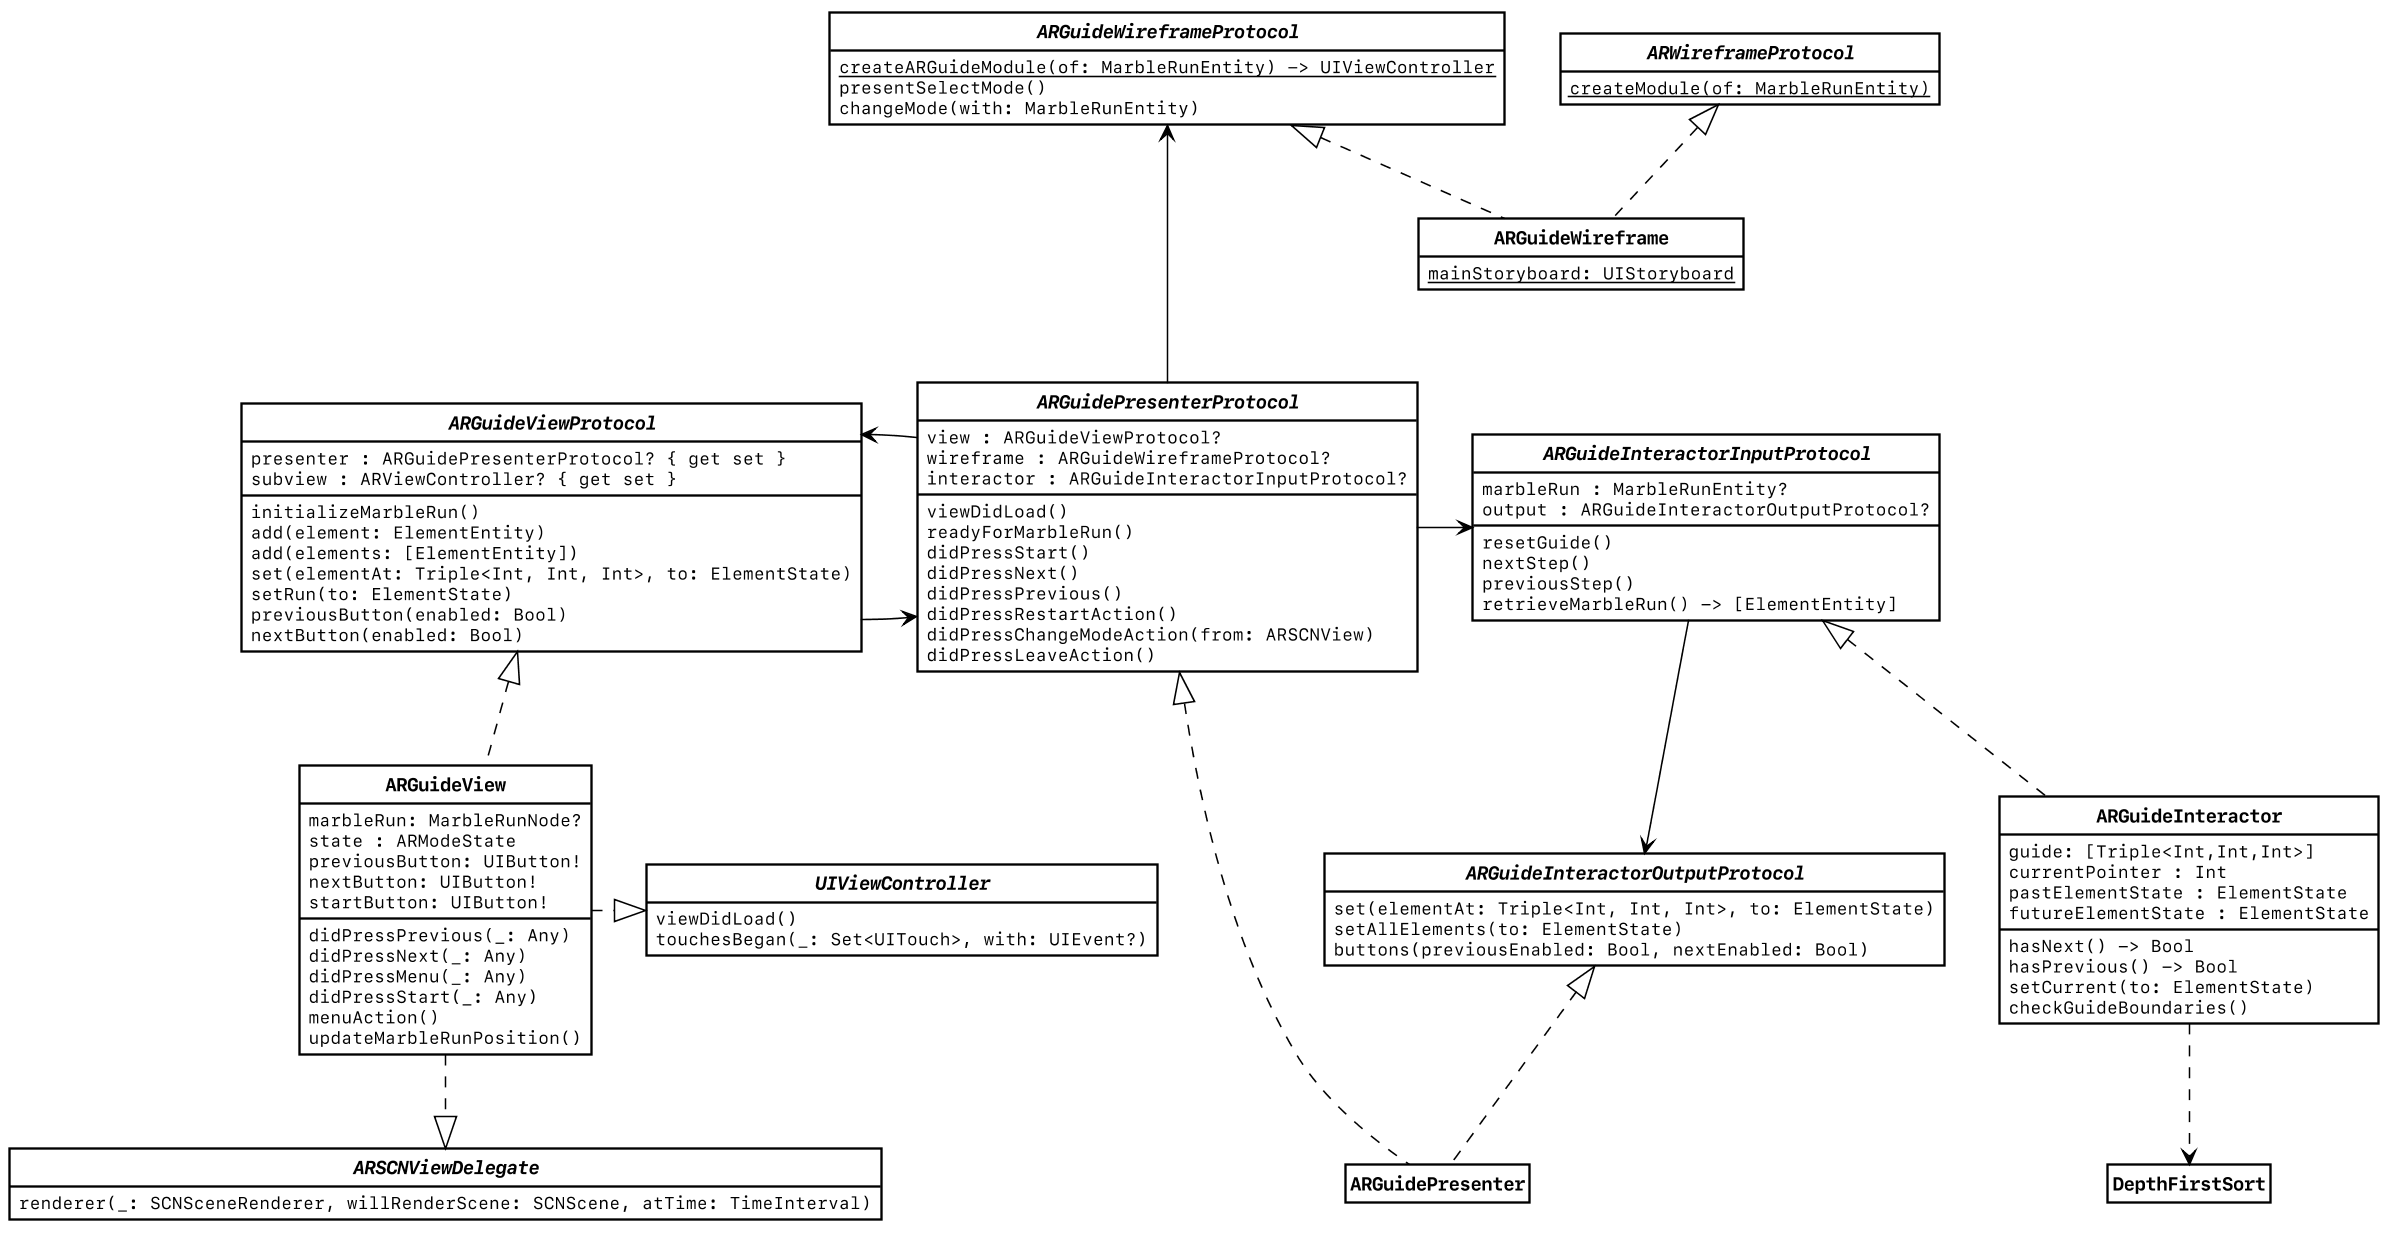
\includegraphics[width=1\textwidth]{classes-arguide}%
	\caption{Klassendiagramm des Moduls "`AR Guide"'}%
	\label{fig:classes-arguide}%
\end{figure}

Das Initialisieren der \texttt{SceneView} und des AR World Tracking übernimmt der \texttt{ARViewController} (siehe \ref{subsub:umsetzung-arviewcontroller}).
Sobald der Benutzer eine erkannte Fläche gewählt hat, übernimmt die \texttt{ARGuideView} die weiteren Aktionen und teilt dem Presenter mit, dass sie bereit ist, die Kugelbahn darzustellen.
Der Presenter fragt vom Interactor die Elemente der Kugelbahn an und fügt sie der View zu.
In \texttt{InitializeMarbleRun} der View wird eine \texttt{MarbleRunNode} erstellt und der Szene hinzugefügt, Elemente werden dann als Kindknoten der Kugelbahn ergänzt.
Die Positionierung der Kugelbahn erfolgt nach dem in Prototyp \ref{subsub:prot-kugelbahn} erarbeiteten Prinzip.

Ist die Position der Kugelbahn fixiert und der Startbutton wird gedrückt, lässt der Interactor von \texttt{DepthFirstSort} die Bauanleitung erstellen (siehe \ref{subsub:umsetzung-depthfirst}).
Der Rückgabewert ist ein Array von Koordinaten, in der Reihenfolgen, in der sie abgearbeitet werden sollen.
Mittels Vor- und Zurück-Buttons kann der Benutzer in der Anleitung navigieren.
Diese Aktionen erhöhen oder verringern im Interactor den \texttt{currentPointer}, der auf die aktuelle aktive Koordinate im Array \texttt{guide} zeigt.

Die View hat keine Kenntnisse über die Anleitung, sondern erhält als Reaktion auf Benutzerinteraktionen vom Presenter mit der Methode \texttt{set(elementAt:to:)} Anweisungen, welche Elemente der Kugelbahn welchen Status erhalten sollen.
So wird beispielsweise das aktive Element der Bauanleitung mit \texttt{ElementState.highlighted} hervorgehoben.

Als einziges Modul in diesem Projekt, nutzt der AR Editor für den Interactor ein Eingabe und Ausgabe Protokoll.
Während das \texttt{ARGuideInteractorInputProtocol} wie bei anderen Modulen vom Presenter genutzt wird um den Interactor anzusprechen, ist \texttt{ARGuideInteractorOutputProtocol} für die umgekehrte Richtung zuständig.

% TODO: Menu Action?

\subsubsection{AR Editor} \label{subsub:umsetzung-modul-areditor}

Im \texttt{AREditor} Modul wird die gewählte Kugelbahn in Augmented Reality bearbeitbar gemacht.
Abbildung \ref{fig:classes-areditor} zeigt das Klassendiagramm des Moduls.

Beim Laden der View werden die Gesten Tap, Long Press und Swipe mit den jeweiligen Eventhandler hinzugefügt.
Wie bei \texttt{ARGuide} übernimmt die Initialisierung der \texttt{SceneView} und von ARKit der \texttt{ARViewController}.
Auch die Positionierung der Kugelbahn läuft nach dem selben Muster.

Nachdem die Position der Kugelbahn fixiert wurde, kann der Editiermodus mit dem Startbutton gestartet werden.
Damit wird der \texttt{state} auf \texttt{ARModeState.editorMode} gesetzt.

\begin{figure}[htb!]
	\centering
	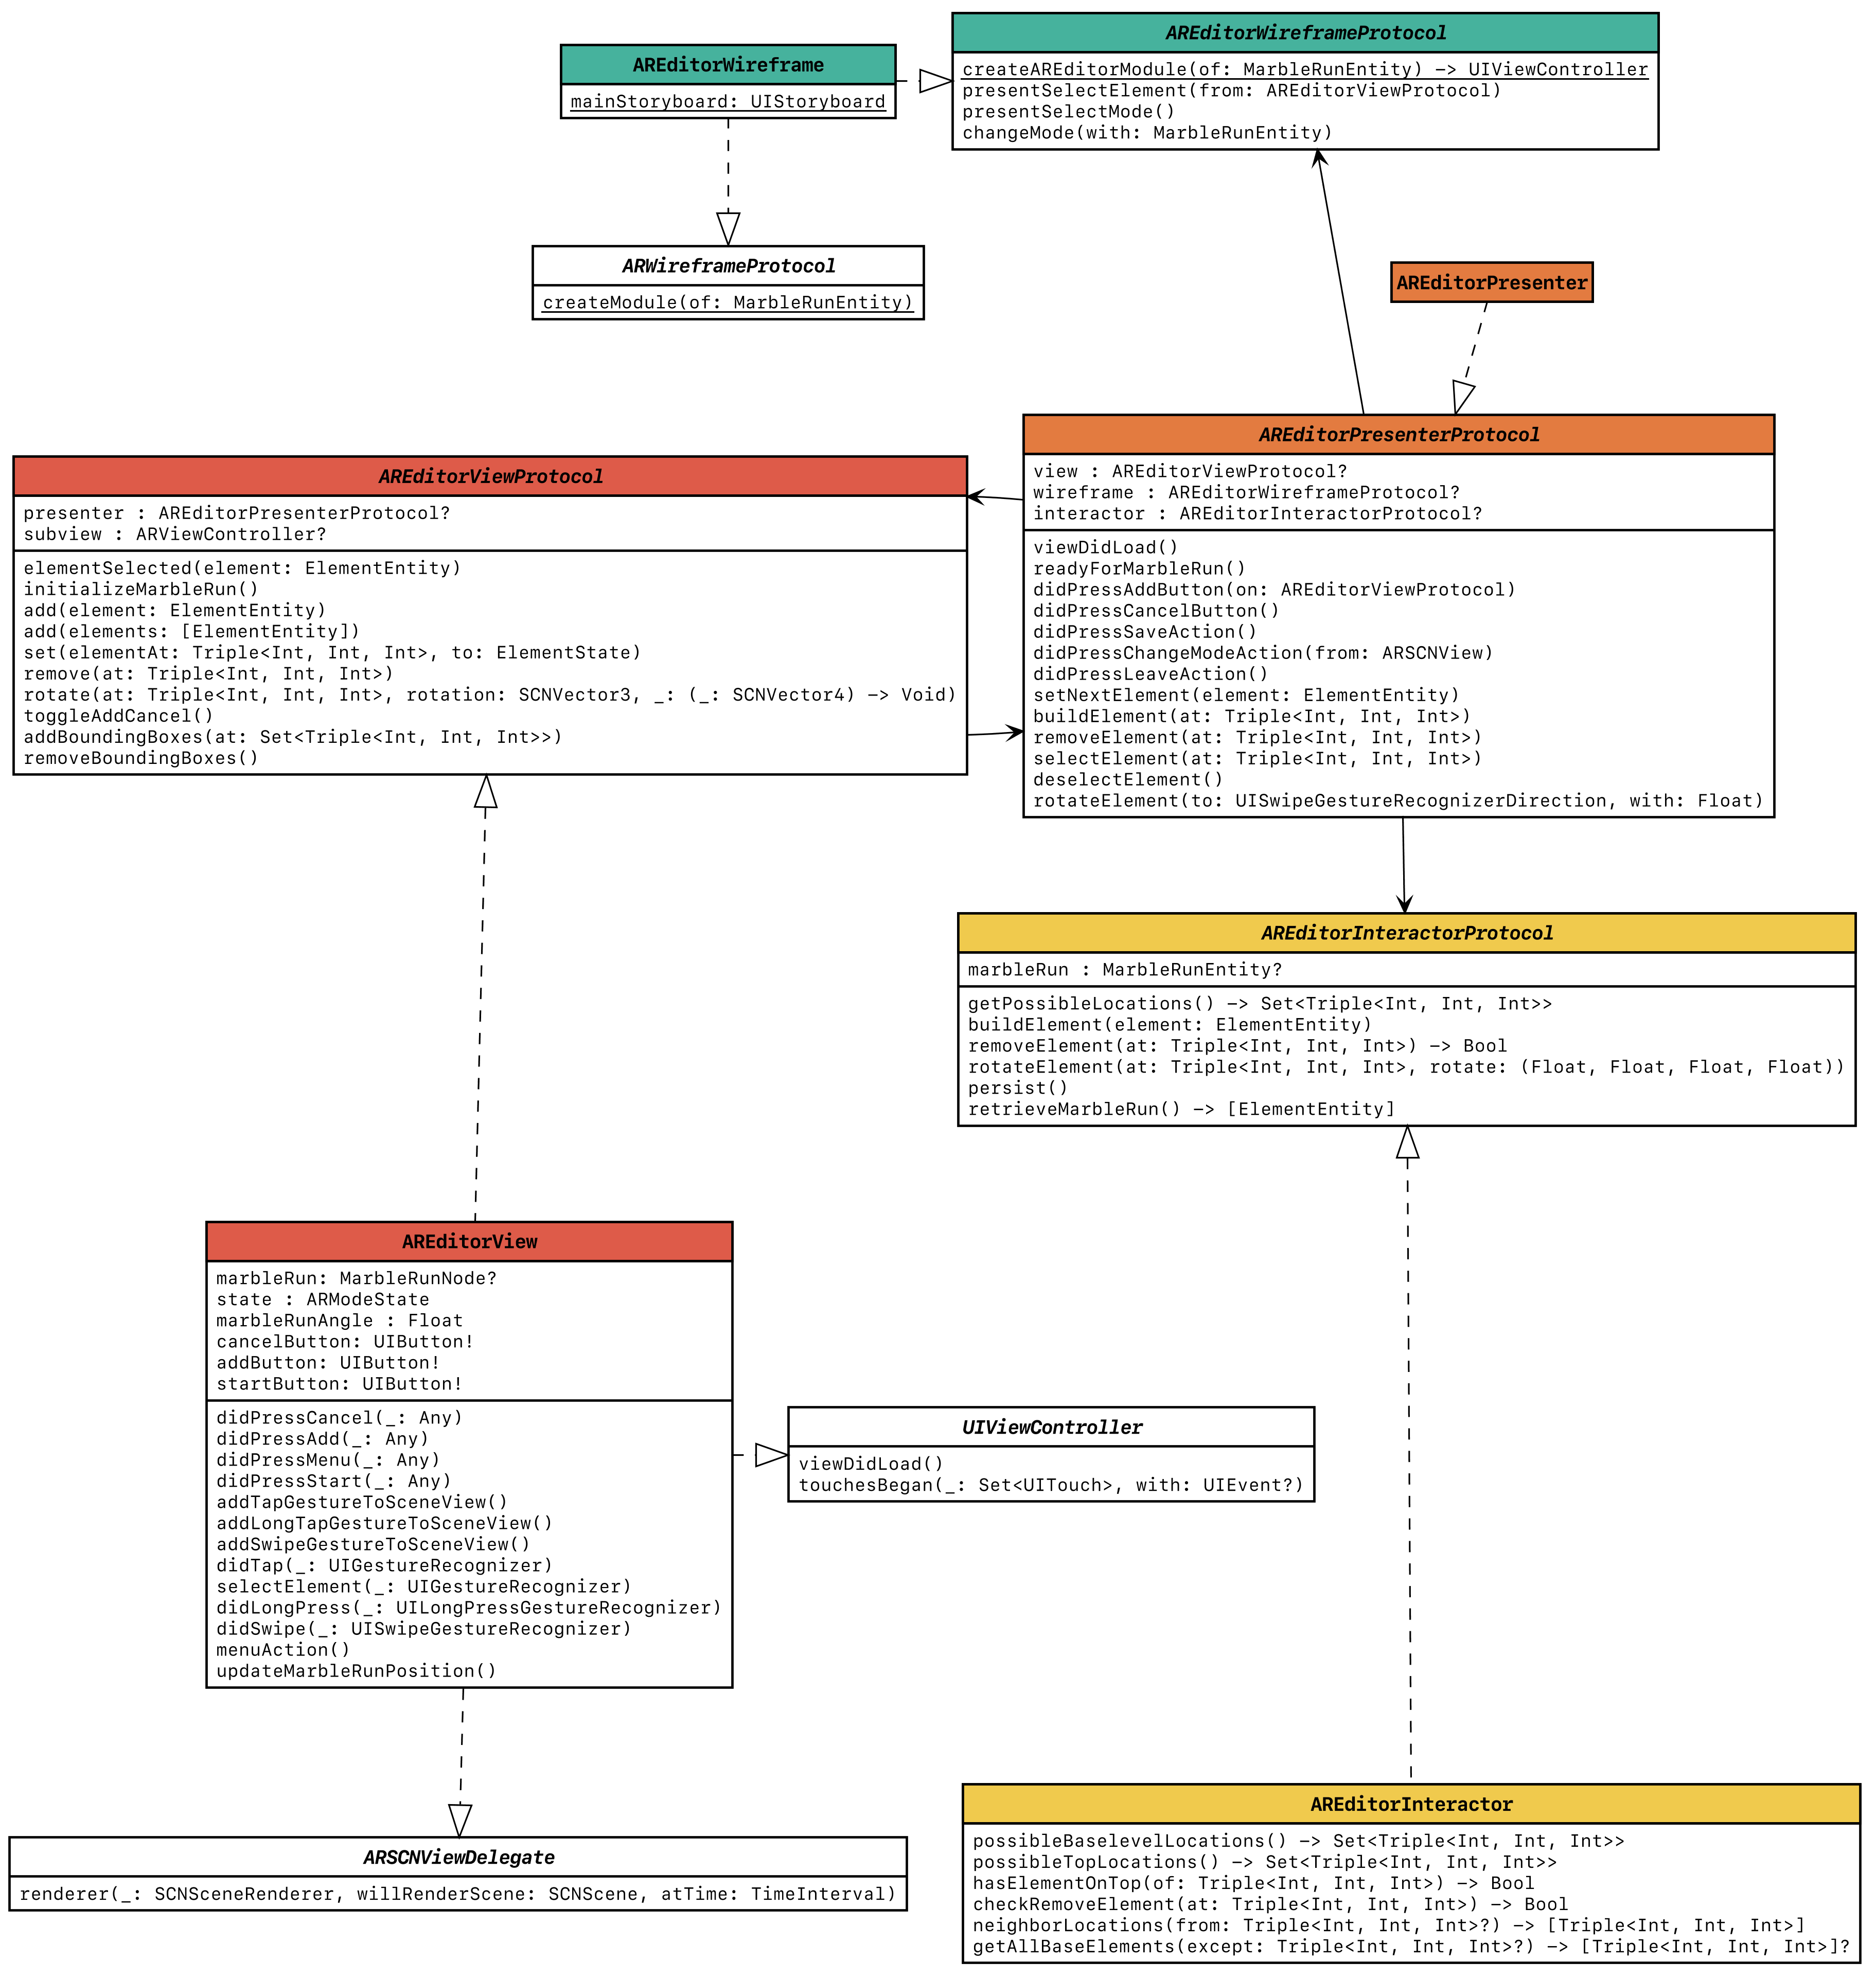
\includegraphics[width=1\textwidth]{classes-areditor}%
	\caption{Klassendiagramm des Moduls "`AR Editor"'}%
	\label{fig:classes-areditor}%
\end{figure}

\textbf{Neues Element hinzufügen} \\
Bei einem Druck des \texttt{addButton} wird das Modul \texttt{ElementList} aufgerufen, von dem die View schliesslich den selektierte Elementtyp durch die Methode \texttt{elementSelected(element:)} erhält.
Dem Presenter wird diese Information weitergeben und dieser fragt beim Interactor nach den möglichen Positionen, an denen das Element platziert werden kann.
Der Interactor sucht einerseits nach allen Koordinaten auf der untersten Ebene der Kugelbahn, die an ein existierendes Element angrenzen und noch leer sind (Methode \texttt{possibleBaselevelLocations()}).
Andererseits wird in \texttt{possibleTopLocations()} nach Elementen gesucht, auf denen noch kein Element steht.
Diese Kriterien führen dazu, dass die Bahn physikalisch möglich ist (keine schwebeden Elemente) und zusammenhängend ist (nur angrenzende Positionen).

All diese Positionen werden als \texttt{BoundingBoxNode} der View hinzugefügt und dargestellt.
Tippt der Benutzer auf einer der Boxen, wird diese mit dem zuvor gewählten Elementtyp ersetzt und alle anderen Positions-Boxen werden wieder ausgeblendet.
Der Presenter gibt dabei die \texttt{ElementEntity} mit aktualisierten Koordination sowohl an den Interactor als auch an die View.

Der Ablauf für den Benutzer um ein Element hinzuzufügen wird in Abbildung \ref{fig:armarblerun-screenshots-editor} in den einzelnen Schritten dargestellt.

\bild{1}{armarblerun-screenshots-editor}{Screenshots der Demo-App: Schritte beim Hinzufügen eines Elements}

\textbf{Element löschen} \\
Die Methode \texttt{didLongPress(\_:)} macht auf die SceneKit Szene einen Hit-Test.
Wenn das Resultat des Hit-Tests ein Kugelbahn Element ist, wird beim Presenter die Methode \texttt{removeElement(at:)} aufgerufen.
Damit wird versucht das entsprechende Element beim Interactor zu entfernen.
Der Interactor überprüft in der Methode \texttt{removeElement(at:)}, ob das Element überhaupt entfernt werden darf.
Dazu darf sich als erstes kein Element darüber befinden.

Wenn sich das Element auf der untersten Ebene der Kugelbahn befindet, dürfen mit dessen Löschung auch keine "`Inseln"' entstehen, sprich die Kugelbahn soll zusammenhängend bleiben.
Das wird in \texttt{checkRemoveElement(at:)} überprüft, indem ausgehend von einem beliebigen Element eine Tiefensuche via direkte Nachbarschaften durchgeführt wird.
Das zu entfernende Element wird dabei ausgelassen.
So werden angrenzende Elemente so lange zur Liste der besuchten Elemente hinzugefügt, bis keines mehr gefunden wird, das nicht bereits besucht wurde.
Eine durch die Löschung entstehende Lücke führt dazu, dass nicht alle Elemente der untersten Ebene besucht werden können.
Deshalb wird am Ende die Anzahl besuchter Elemente mit der Gesamtzahl der verbleibenden Elemente in der untersten Ebene verglichen.
Sind die beiden Zahlen unterschiedlich, hängt die Kugelbahn nach Entfernung des Elements nicht mehr zusammen und der Interactor gibt ein \texttt{false} an den Presenter zurück, der die Löschung abbricht.

\textbf{Element rotieren} \\
Wird ein Element durch Antippen ausgewählt, wird es hervorgehoben und der Presenter merkt es sich als \texttt{selectedElement}.
Ist das Attribut gesetzt und eine Swipe Geste wird ausgeführt, wird das Element in Richtung der Geste rotiert.
Die View berechnet den Winkel zwischen Kamera und Ausrichtung der Kugelbahn und gibt diesen zusammen mit der Richtung der Geste an die Presenter Methode \texttt{rotateElement(to:with:)}.
Es wird je nach Swipe-Richtung ein Vektor erstellt, der die Achse und Richtung der Rotation beschreibt.
Für einen Swipe nach links ist dies beispielsweise der Vektor \texttt{SCNVector3(0, -1, 0)} zur Rotation um die y-Achse.
Die korrekte Achse für vertikale Swipes ist abhängig vom Betrachtungswinkel.
Daher wird dort anhand des erhaltenen Winkels entweder die x- oder z-Achse mit einem positiven (1) oder negativen (-1) Wert belegt.

Ist die Rotation berechnet, wird der \texttt{rotation} Vektor in der View genutzt um auf dem ausgewählten Element eine Rotations-Aktion auszuführen, die wie folgt definiert wird:
\mint[style=xcode,breaklines]{swift}{let action = SCNAction.rotate(by: .pi/2, around: rotation, duration: 0.2)}
So wird das Element innert 0.2 Sekunden um 90° um die im Vektor definierte Achse rotiert.
Dabei bleibt das Koordinatensystem erhalten.

Das in Prototyp \ref{subsub:prot-interagieren} erarbeitete Vorgehen mit \texttt{SCNAction.rotateBy(x:y:z:rotation:)} und dem Zurücksetzen der Orientierung mit \texttt{SCNQuaternion}, erwies sich als Trick, der für die Demo-App nicht verwendet werden konnte.
Für einen Würfel, dessen Seiten alle gleich sind, funktioniert das Vorgehen zwar.
Aber die hier verwendeten Elemente zeigten, dass sich der Würfel nach der Rotation jeweils in den Originalzustand zurück versetzt. 

\subsubsection{Element List} \label{subsub:umsetzung-modul-elementlist}

Das \texttt{ElementList} Modul listet alle verfügbaren Elementtypen auf, die der aktuell bearbeiteten Kugelbahn hinzugefügt werden können.
Es ist ähnlich dem \texttt{MarbleRunList} Modul.
Abbildung \ref{fig:classes-elementlist} zeigt das Klassendiagramm des Moduls.

\bild{1}{classes-elementlist}{Klassendiagramm des Moduls "`Element List"'}

Die \texttt{ElementListView} wird modal vom AR Editor dargestellt.
Sie meldet ihre Bereitschaft an den Presenter, der vom Interactor die Liste der Elementtypen abfragt.
Der Interactor greift dann wie folgt auf die SceneKit Scene mit den cuboro Elementen zu:
\mint[style=xcode,breaklines]{swift}{let cubes = SCNScene(named: "art.scnassets/cuboro-set.scn")?.rootNode}
Aus den Kindknoten von \texttt{cubes} stellt der Interactor ein Array von \texttt{ElementEntity} zusammen und gibt es als Rückgabewert dem Presenter zurück.
Dies wird an die View weitergegeben, welche daraus wie \texttt{MarbleRunList} ihre Collection View aufbaut.

Bei der Wahl eines Elementtyps durch den Benutzer ruft die View \texttt{didSelect(element:on:)} beim Presenter auf, was dieser an das Wireframe weitergibt.
Das Wireframe lässt die View ausblenden und gibt das selektierte Element an den AR Editor weiter.

\subsection{Persistenz}

\subsubsection{Data Manager} \label{subsub:umsetzung-datamanager}

Der Data Manager übernimmt das Lesen und Schreiben von persistierten, bzw. zu persistierenden Daten.
In dieser Demo-App sind dies die Kugelbahnen, bestehend aus einer \texttt{MarbleRunEntity} und ihrer \texttt{ElementEntity}s.
Der \texttt{MarbleRunDataManager} bietet statische Methoden zum Lesen aller Kugelbahnen (\texttt{retrieveMarbleRunList()}), Schreiben einer Kugelbahn (\texttt{persist(\_:)}) und einer Überprüfung, ob überhaupt gespeicherte Kugelbahnen vorhanden sind (\texttt{isDirectoryEmpty()}).

Als Dateiablage wird der Dokumentenordner des iOS Dateisystem mittels \texttt{FileManager} genutzt.
Die \texttt{MarbleRunEntity} jeder Kugelbahn wird mittels \texttt{NSKeyedArchiver} in einer eigenen Datei gespeichert:
\mint[style=xcode,breaklines]{swift}{NSKeyedArchiver.archiveRootObject(run, toFile: filePath.path)}
Damit dies möglich ist, müssen die Entitäten von \texttt{NSObject} erben und das \texttt{NSCoding} Protokoll adoptieren (Kapitel \ref{subsub:umsetzung-entities-nodes}).

\subsubsection{Entitäten und Nodes} \label{subsub:umsetzung-entities-nodes}

Die beiden zentralen Datenobjekte im Projekt sind Kugelbahnen und deren Elemente.
Sie werden für die Darstellung in der AR Szene aber auch zur Persistierung im Dateisystem gebraucht.
Aufgrund der VIPER Architektur wurden diese beiden Aspekte auch entsprechend getrennt.
Einerseits gibt es die \textbf{Nodes}, die von \texttt{SCNNode} erben und Informationen zur Geometrie und Erscheinungsbild haben.
Sie werden daher nur in den Views von AR Guide und AR Editor verwendet.
Anderersetis sind die \textbf{Entities} schlanke Klassen, die im Rest der App genutzt werden und persistiert werden können.

\textbf{Nodes} \\
Alle Nodes erben von der Klasse \texttt{SCNNode} und können so direkt in SceneKit verwendet und dargestellt werden.

\begin{description}
	\item[PlaneNode] ist zur Darstellung von durch ARKit erkannten Flächen. Sie hat eine \texttt{update} Methode, damit sie bei Änderungen der Grösse und Position aktualisiert werden kann.
	\item[BoundingBoxNode] ist ein einfacher Würfel, wie er als \texttt{BasicCube} in verschiedenen Prototypen verwendet wurde. Objekte dieses Typs werden im AR Editor zur Anzeige möglicher Positionen eines neuen Elements verwendet.
	\item[ElementNode] ist die Node für einzelne Kugelbahn Elemente. Sie hat eine \texttt{Triple} Location, einen Status vom Typ \texttt{ElementState} und einen Type, der ihre Geometrie definiert. Abhängig vom Status wird das Erscheinungsbild der Node verändert. Bei der Instanziierung wird basierend auf dem Type die Geometrie aus der SceneKit Scene "`cuboro-set.scn"' geladen. Die Position eines Elements wird mit \texttt{Triple} Koordinaten als relative Position zum Kugelbahn Ursprung in Anzahl Elemente definiert (\ref{subsub:umsetzung-triple}). Die reale Position wird durch die Multiplikation mit der Seitenlänge der Elemente berechnet.
	\item[MarbleRunNode] dient als Basisnode, der \texttt{ElementNode} Objekte hinzugefügt werden. Sie bietet Methoden, um sich mit \texttt{SCNBillboardConstraint} stets zur Kamera auszurichten, wie in Prototyp \ref{subsub:prot-kugelbahn} und Code \ref{code:prot-kugelbahn-billboardconstraint} gezeigt.
\end{description}

\textbf{Entities} \\
Die beiden Entitäten \texttt{MarbleRunEntity} und \texttt{ElementEntity} adoptieren das \texttt{NSCoding} Protokoll, um sie im Dateisystem zu persistieren.
Das Protokoll verlangt zwei Methoden – \texttt{init?(coder:)} und \texttt{encode(with:)} – in denen alle zu persistierenden Attribute kodiert, beziehungsweise dekodiert, werden müssen.


\subsection{Storyboard}

\bild{1}{project-storyboard}{Das Storyboard des Projekts}

Abbildung \ref{fig:project-storyboard} zeigt das Storyboard des Projekts.
Dort ist links der Startbildschirm (Abschnitt \ref{subsub:umsetzung-modul-selectmode}) mit Navigation Controller und einem Segue auf den Informationsbildschirm definiert.
In der Mitte sind die beiden Collection Views für die Kugelbahnen (\ref{subsub:umsetzung-modul-marblerunlist}) und die Elementtypen (\ref{subsub:umsetzung-modul-elementlist}).
Auf der rechten Seite sind die beiden AR Views mit dem \texttt{ARViewController} (\ref{subsub:umsetzung-arviewcontroller}), auf den sie in einer Container View verweisen.


\subsection{Weitere Bestandteile}

\subsubsection{Triple} \label{subsub:umsetzung-triple}
Das Struct Triple beinhaltet ein Tupel mit drei Elemente. Tripel adoptiert das Hashable Protokoll um auch in einem Set verfügbar zu sein.

Das Triple wird dazu verwendet die relativen Koordinaten der Kugelbahn Elemente festzuhalten. Anhand dieser Koordinaten können Berechnungen zwischen den Elementen durchgeführt werden wie z.B. Die benachbarten Elemente gefunden werden.

\subsubsection{DepthFirstSort} \label{subsub:umsetzung-depthfirst}

Die \texttt{DepthFirstSort} Klasse sortiert ein Array von Triple nach dem Prinzip der Tiefensuche so, dass das resultierende Array für die Bauanleitung verwendet werden kann.
Die grundlegende Methode entspricht der in Prototyp \ref{subsub:prot-kugelbahnaufbau2} erarbeiteten Lösung des \texttt{TrackBuilder}, ist aber in dieser Klasse mit einer rekursiven Methode implementiert.

Dem Konstruktor wird das zu sortierende Array mitgegeben und mit der Methode \texttt{generate} wird das sortierte Array generiert und zurückgegeben.
Die \texttt{search(from:)} Methode ergänzt das erhaltene Triple zum Resultat und ruft sich rekursiv selber für jedes Nachbarelement auf.
Diese Suche wird auf jeder Ebene durchgeführt bis alle Elemente erfasst wurden.

\subsubsection{ARViewController} \label{subsub:umsetzung-arviewcontroller}

Im \texttt{ARViewController} werden die für beide AR Modi identischen Initialisierungsabläufe für Augmented Reality behandelt.
Darin wird die \texttt{ARSession} konfiguriert und die Flächenerkennung und -bestimmung durchgeführt, wie in Prototyp \ref{subsub:prot-overlay} entwickelt.
Bei aktiviertem Debug Mode wird die Statistiken und weitere Debug Optionen der Scene View aktiviert.
So wird dann der World Origin (Ursprungspunkt der Weltkoordinaten) und Feature Punkte des Tracking angezeigt.

\subsubsection{Informationsbildschirm}
Oben rechts auf dem Startbildschirm befindet sich ein Informationsicon mit dem der Informationsbildschirm eingeblendet werden kann. Dieser zeigt die aktuelle Version, Entwickler, Abhängigkeiten und dass die App als Resultat der Industrieprojektarbeit an der Fachhochschule Luzern entstanden ist. Zusätzlich kann der Debug Modus aktiviert werden um Laufzeitinformationen der AR View zu erhalten. Ob der Debug Modus aktiviert ist, wird in den User Defaults gespeichert.
